\documentclass[12pt]{beamer}
\usepackage[utf8]{inputenc}
\usepackage[T1]{fontenc}
\usepackage{lmodern}
\usepackage[spanish]{babel}
\usepackage{amsmath}
\usepackage{amsfonts}
\usepackage{amssymb}
\usepackage{graphicx}
\usepackage{hyperref}
\usepackage{enumitem}
\usepackage{etoolbox} % to reduce spacing in bearmers toc
\usetheme[block=fill, subsectionpage=simple]{metropolis}

% to reduce spacing in bearmers toc
\makeatletter
\patchcmd{\beamer@sectionintoc}
{\vfill}
{\vskip\itemsep}
{}
{}
\makeatother

\begin{document}
	\author{Fernando Oleo Blanco \\ fernando.oleo@alu.comillas.edu \hfill 	\href{https://github.com/Irvise/Documents}{github.com/Irvise/Documents}}
	\title{Introducción a la simulación}
	%\subtitle{}
	%\logo{}
	%\institute{ICAI - LinuxEC}
	\date{\today}
	%\subject{}
	%\setbeamercovered{transparent}
	\setbeamertemplate{navigation symbols}{}
	\setbeamertemplate{footline}[page number]
\begin{frame}[plain]
	\maketitle
\end{frame}

\begin{frame}{Información de la charla}
	\textbf{Duración estimada:} 2:30h \\
	\textbf{¡Haremos una simulación!} Así que por favor, celeridad
	
	\begin{block}{Esta charla no tratará}
		\begin{itemize}
			\item ANSYS \textregistered\ o ningún software en específico
			\item Métodos numéricos ni principios de convergencia
			\item Funcionamiento de los simuladores ni sus fundamentos
			\item Análisis de sensibilidad ni optimizaciones de ningún tipo
			\item Mallado (meshing) de manera formal
			\item Diseño 3D, esto ya lo deberíais traer
			\item Puede que no de tiempo al caso práctico de post-procesado
		\end{itemize}
	\end{block}
\end{frame}

\begin{frame}{Índice}
	\setcounter{tocdepth}{2}
	\tableofcontents
\end{frame}

\section{Qué es la simulación y qué se requiere}

\begin{frame}{Requisitos mínimos para simular}
	\begin{block}{Entender muy, muy bien la física/ingeniería del problema}
		Los ordenadores no son tan inteligentes. Es un requisito indispensable entender muy bien lo aprendido en las clases. \textbf{Dadle valor a la ingeniería.}
	\end{block}
	Otros:
	\begin{itemize}
		\item Ganas. Los errores son constantes
		\item Leer la documentación. Hacer cursos/ver vídeos
		\item Práctica
	\end{itemize}
\end{frame}

\begin{frame}{¿Qué es la simulación?}
	Una simulación como su nombre indica, no es la realidad. \\~
	
	\begin{block}{La simulación es una aproximación a la realidad}
		La calidad de la aproximación depende de la persona que la realice y de su trabajo; los conocimientos sobre la materia, el simulador y, sobretodo, la precisión que nosotros queramos darle.
	\end{block}	
\end{frame}

\begin{frame}{Escala dimensional ¡y temporal! de la simulación I}
	\begin{figure}
		\centering
		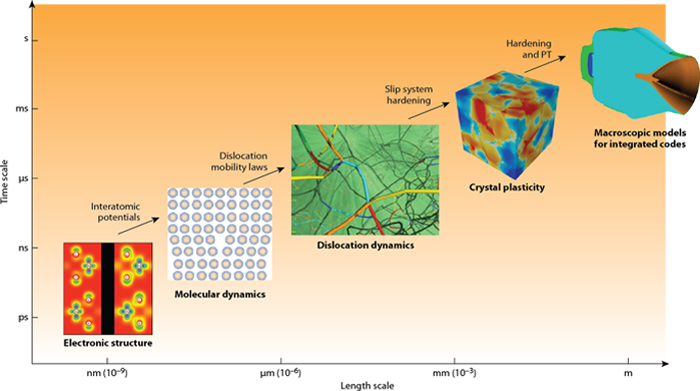
\includegraphics[width=1\linewidth]{ms11}
		\caption{Escala temporal y espacial de simulación. Fuente: \href{https://manufacturing.llnl.gov/content/assets/images/ms/ms11.jpg}{LLNL}}
		\label{fig:ms11}
	\end{figure}
\end{frame}

\begin{frame}{Escala dimensional ¡y temporal! de la simulación II}
	\begin{figure}
		\centering
		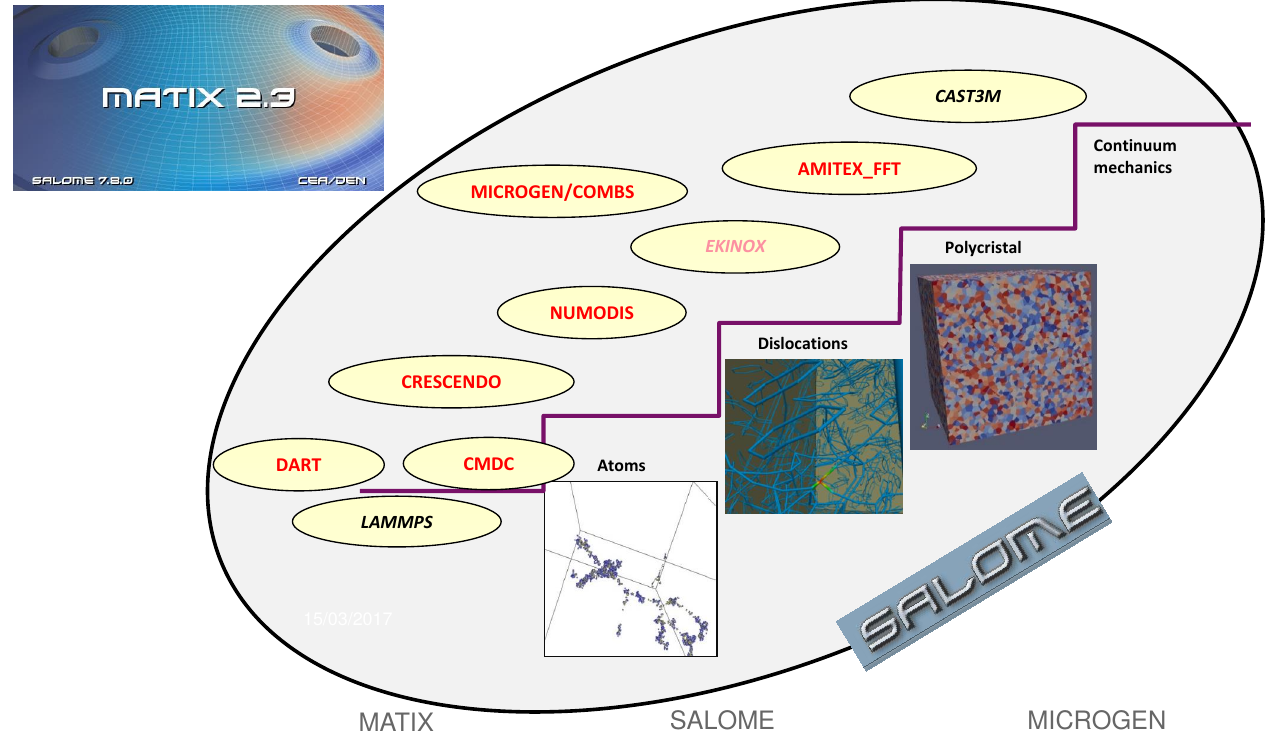
\includegraphics[width=1\linewidth]{cea_simulation_scale}
		\caption{Otro ejemplo, esta vez, con software específico. Fuente: presentación de MATIX\_P, CEA}
		\label{fig:ceasimulationscale}
	\end{figure}
	
\end{frame}

\section{Software de simulación comercial}

\begin{frame}{Selección de software para la simulación}
	Solo dos comentarios:
	\begin{block}{¡Cuidado con las licencias!}
		Las licencias de los programas a los que os da acceso la universidad son de carácter educacional. Esto significa que no podéis hacer nada comercial con ese software.
	\end{block}
	\pause
	\begin{block}{Selección de software}
		Por lo general no tendréis que elegir el programa para simular, ya os vendrá dictado por la empresa o institución. Sin embargo, si es para uso propio u os toca elegir, \textbf{haced siempre un estudio del mercado.} A continuación os dejo una pequeña ayuda.
	\end{block}
\end{frame}

\begin{frame}{Algunos criterios de selección}
	\begin{itemize}[label=$\checkmark$]
		\item Que pueda simular lo que se desea
		\item Eficiente
		\item Flexible (el software libre gana claramente)
		\item Escalable. ¿Y si mañana quiero optimizar?
		\item Integración con otro software que pueda ser necesario (el software de pago es muy bueno en esto)
		\item Costes
	\end{itemize}
\end{frame}

\subsection{Software de pago}

\begin{frame}{Una pequeñísima selección}
	\begin{columns}
		\begin{column}{0.5\textwidth}
			Los más conocidos:
			\begin{itemize}
				\item \href{https://www.ansys.com}{ANSYS \textregistered}
				\item \href{https://www.mscsoftware.com}{NASTRAN (MSC) \textregistered}
				\item \href{https://www.comsol.com}{COMSOL Multiphysics \textregistered}
				\item \href{https://solidedge.siemens.com/en/solutions/products/simulation/}{Solid Edge \textregistered}
				\item \href{https://www.solidworks.com/category/simulation-solutions}{SolidWorks \textregistered}
				\item \href{https://www.autodesk.com/solutions/simulation/overview}{Autodesk \textregistered}
				\item \href{https://www.mathworks.com/}{Matlab \textregistered}
				\item $\vdots$
			\end{itemize}
		\end{column}
		\begin{column}{0.6\textwidth}
			Otros interesantes...
			\begin{itemize}
				\item \href{https://www.simscale.com/}{\textbf{Simscale \textregistered. ¡Servicio on-line!}}. Versión gratuita sin ``restricciones''. \href{https://marketing.simscale.com/acton/attachment/14483/f-0336/1/-/-/-/-/SimScale_Simulation_Features_Overview.pdf}{Link para ver capacidades}
				\item \href{https://europlexus.jrc.ec.europa.eu/public/manual_pdf/manual.pdf}{Europlexus \textregistered} \\ Ultrafast-transients, thermal, fluid and mechanical coupling. Aimed towards research
				\item \href{http://www-cast3m.cea.fr/}{Cast 3M \textregistered} \\ Thermo-mechanical. Aimed towards research
			\end{itemize}
		\end{column}
	\end{columns}
\end{frame}

\subsection{Software libre/gratuito}

\begin{frame}{Una pequeña selección}
	Si se desea ver un listado más grande, tengo un pequeño resumen hecho en \textit{\href{https://github.com/Irvise/Documents/blob/master/Cheatsheets/Libre/Packages.md}{link}}, bajo la sección de ingeniería y ciencias.
	\begin{columns}
		\begin{column}{0.6\textwidth}
			\begin{itemize}
				\item \href{https://www.freecadweb.org/}{FreeCAD.} Que el nombre no os eche para atrás, trae de todo y para empezar vais más que sobrados. Tiene plug-ins para interactuar con OpenFOAM
				\item \href{https://openfoam.org/}{OpenFOAM.} Uno de los CFDs más avanzados del mundo. Se usa especialmente en superordenadores e investigación
			\end{itemize}
		\end{column}
		\begin{column}{0.5\textwidth}
			\begin{itemize}
				\item \href{https://code-aster.org/spip.php?rubrique2}{Code\_Aster.} Simulador termo-mecánico, una bestia donde se hayan visto
				\item \href{https://www.code-saturne.org/cms/}{Code\_Saturne.} CFD
				\item \href{http://www.elmerfem.org/blog/}{ElmerFEM.} Multyphysics
				\item $\vdots$
			\end{itemize}
		\end{column}
	\end{columns}
\end{frame}

\begin{frame}{Para terminar...}
	Una de las grandes ventajas del software libre, es que se puede ver y modificar el código. Para proyectos de gran complejidad o poco comunes, modificar el código es casi siempre esencial.
	
	\begin{block}{Documentación}
		Muchos de los programas, en especial los programas libres, tienen toneladas de literatura y ejemplos que pueden ser útiles tanto para su aprendizaje como para la resolución de casos de ingeniería. \href{https://www.code-aster.org/V2/doc/v13/en/index.php?man=R0}{\textbf{Como recomendación, mirad los informes de referencia de Code\_Aster, ver secciones V2 o superior.}}
	\end{block}
\end{frame}

\section{Los cinco principios de toda simulación}

\begin{frame}{Los cinco principios de la simulación}
	\begin{itemize}
		\item Análisis (ingenieril) del problema
		\item Creación de la geometría y grupos
		\item Mallado, \textit{meshing} en inglés (FEA)
		\item Configuración de la simulación. Simulación
		\item Post-procesado
	\end{itemize} \pause
	\begin{block}{Todas son importantes}
		No os saltéis ninguna jamás. Especialmente el análisis y el post-procesado, que son las más olvidadas e importantes.
	\end{block}
	Cada principio requiere del resto, no se realiza uno sin tener claro el resto
\end{frame}

\section{Caso práctico, desarrollo de la teoría}

\begin{frame}{Dinámica de la parte práctica}
	A continuación haremos un caso práctico ``real''. Usaremos el software \href{https://code-aster.org/spip.php?article303}{SALOME-Meca} para la simulación, \href{https://code-aster-windows.com/download/}{\textit{link para Windows}}. \\~
	
	La dinámica del caso es la siguiente:
	\begin{enumerate}
		\item Se introduce la sección teórica
		\item Se ven ejemplos y se comentan. \textbf{¡Participación obligatoria!}
		\item Vamos al programa y aplicamos lo visto
	\end{enumerate}
\end{frame}

\subsection{Presentación y análisis}

\begin{frame}{Análisis}
	Comprobaciones que hacer:
	\begin{itemize}[label=$\checkmark$]
		\item Objetivo de la simulación
		\item Elementos/fuerzas que intervienen
		\item Análisis
		\item Simplificación, equivalencias
		\item Simulación efectiva
	\end{itemize}
	\begin{block}{En resumidas cuentas}
		Ya deberíamos saber cómo serán los resultados antes de simularlo (en la gran mayoría de los casos).
	\end{block}
\end{frame}

\begin{frame}{Caso práctico. El jefe pregunta: ¿Aguanta la viga?}
	\begin{figure}
		\centering
		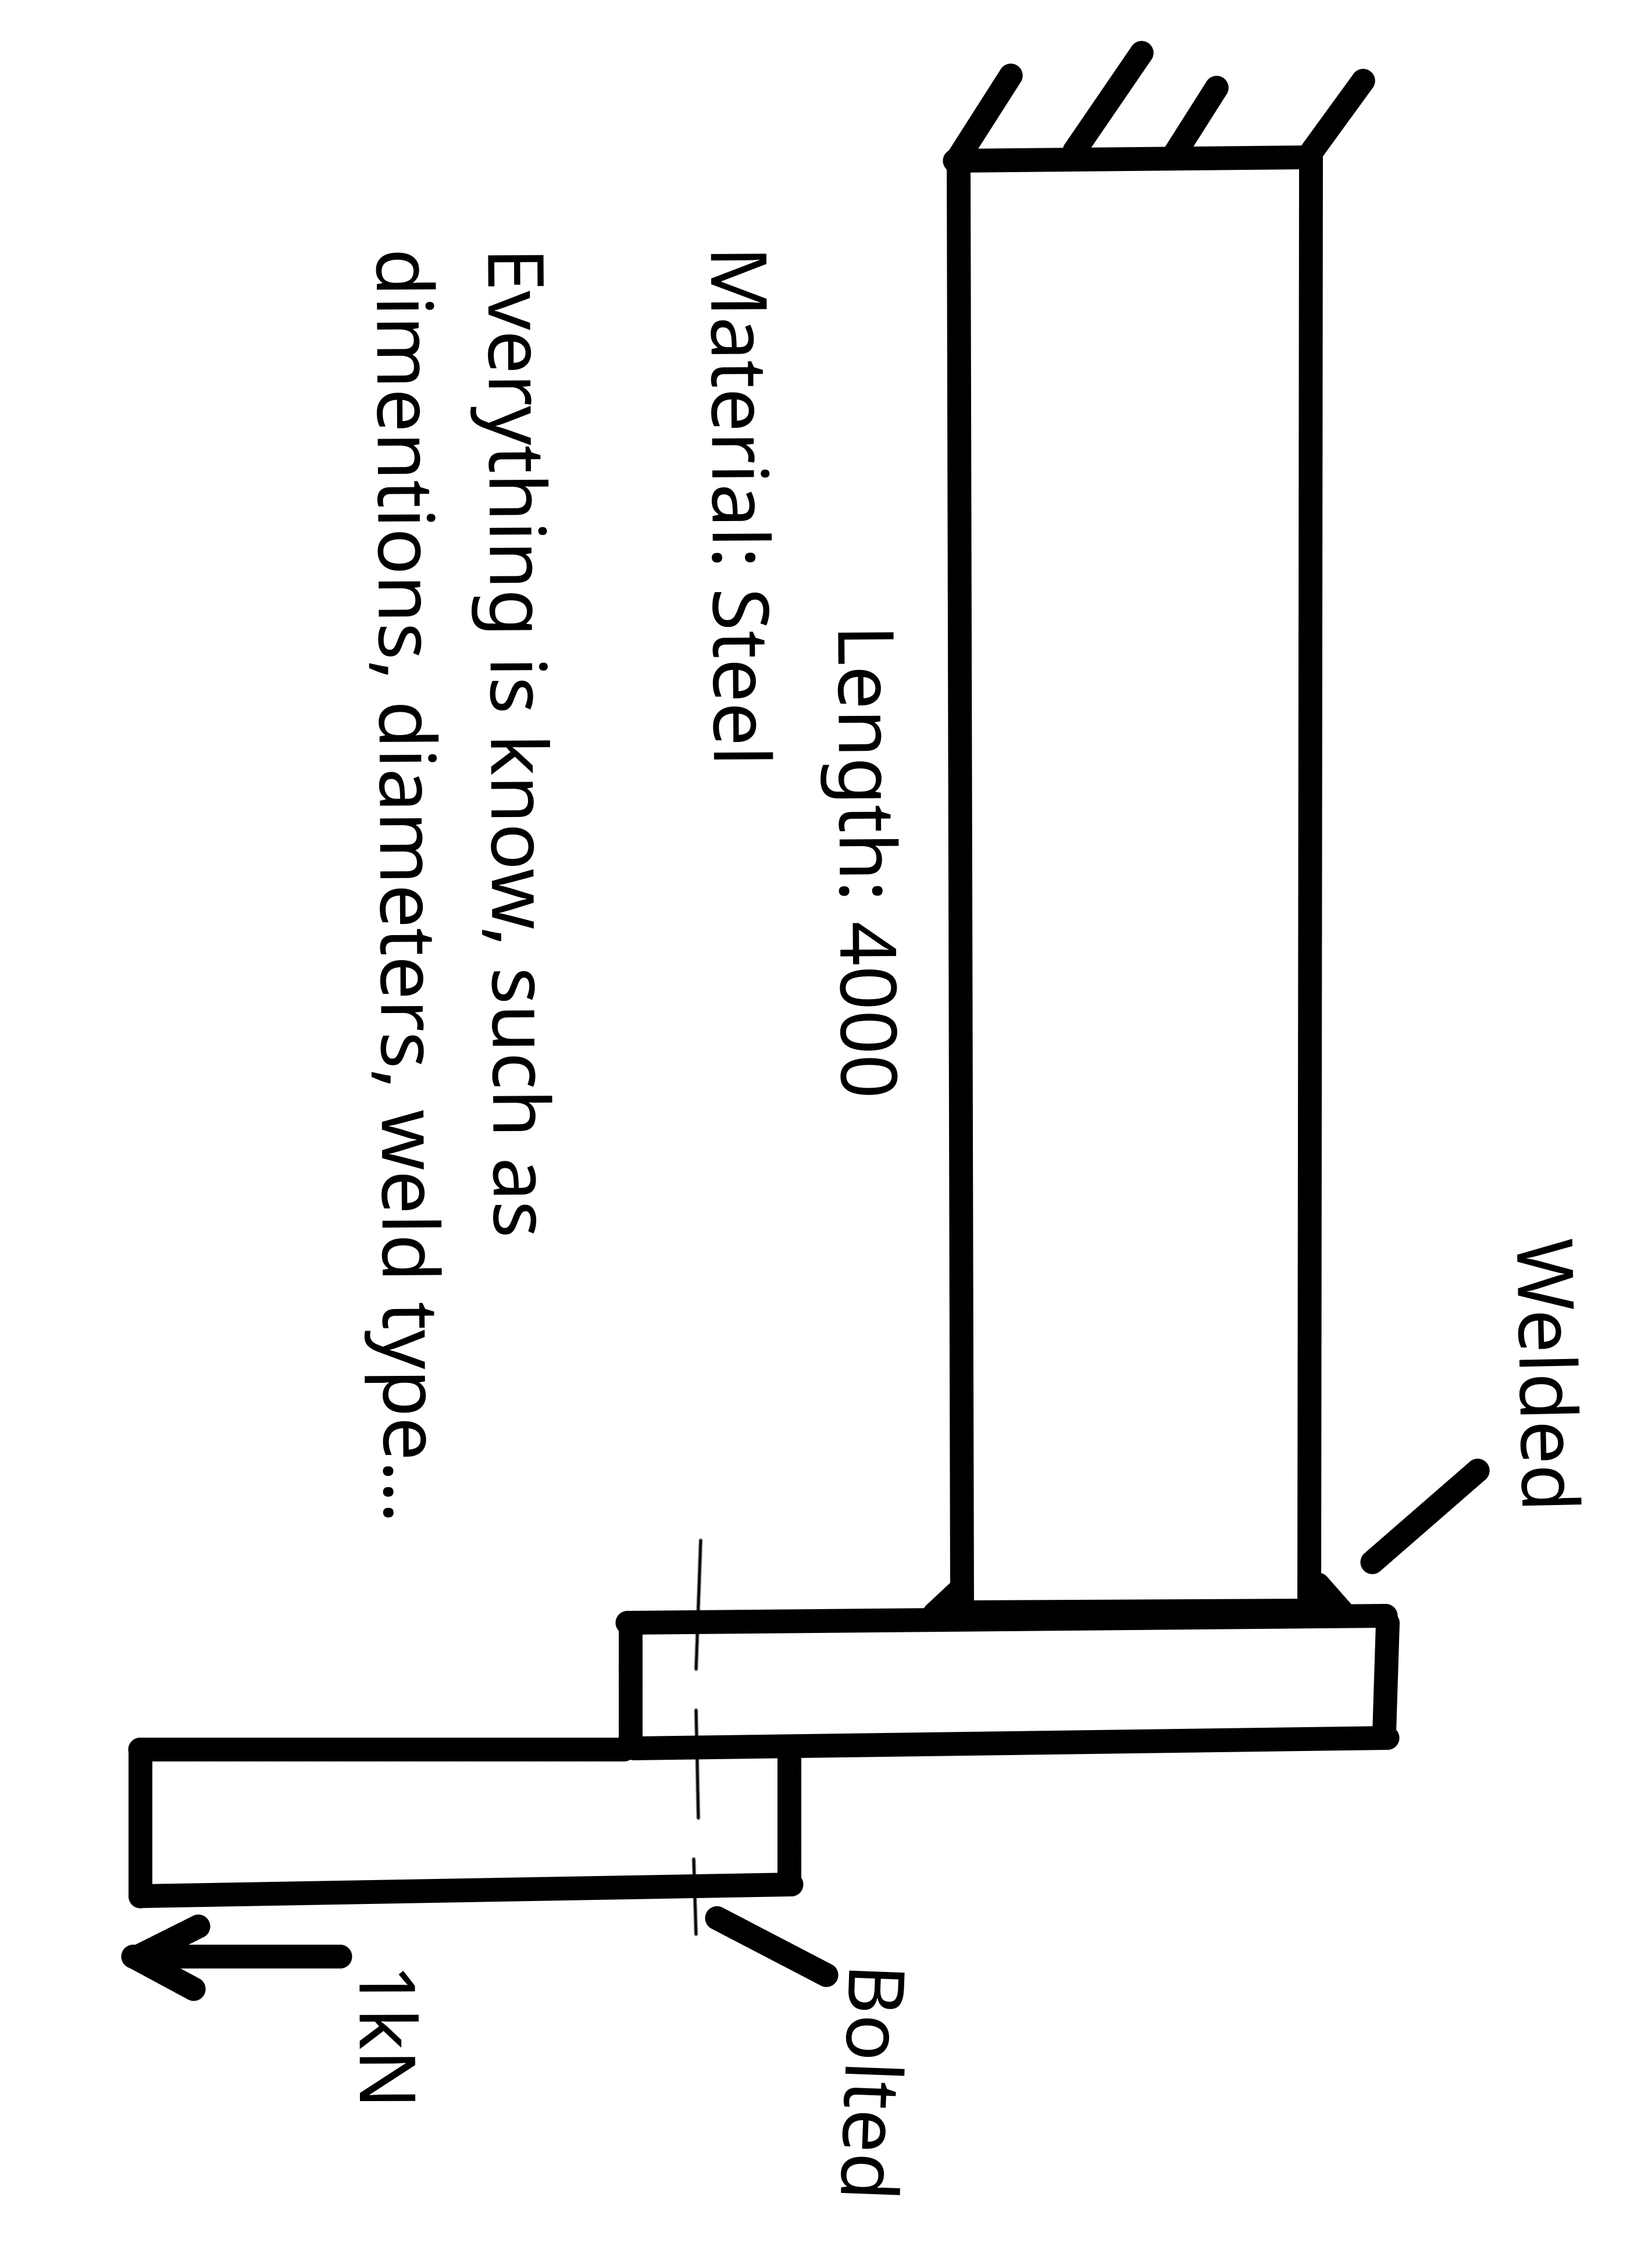
\includegraphics[width=0.7\linewidth,angle=90]{case}
		\label{fig:case}
	\end{figure}
\end{frame}

\begin{frame}{Ejecución del análisis}
	\begin{itemize}[label=$\checkmark$]
		\item Nunca puede romper por la soldadura
		\item Los tornillos se sobredimensionan, su seguridad está asegurada
		\item La pregunta solo se refiere a la viga, nos olvidamos de las planchas metálicas... ¿Aunque sean de 100kg?
		\item La zona más crítica de la viga es en empotramiento
		\item La parte superior tiene que estar a tracción, la inferior a compresión
	\end{itemize}
\end{frame}

\begin{frame}{Sistema simplificado para la simulación}
	\begin{figure}
		\centering
		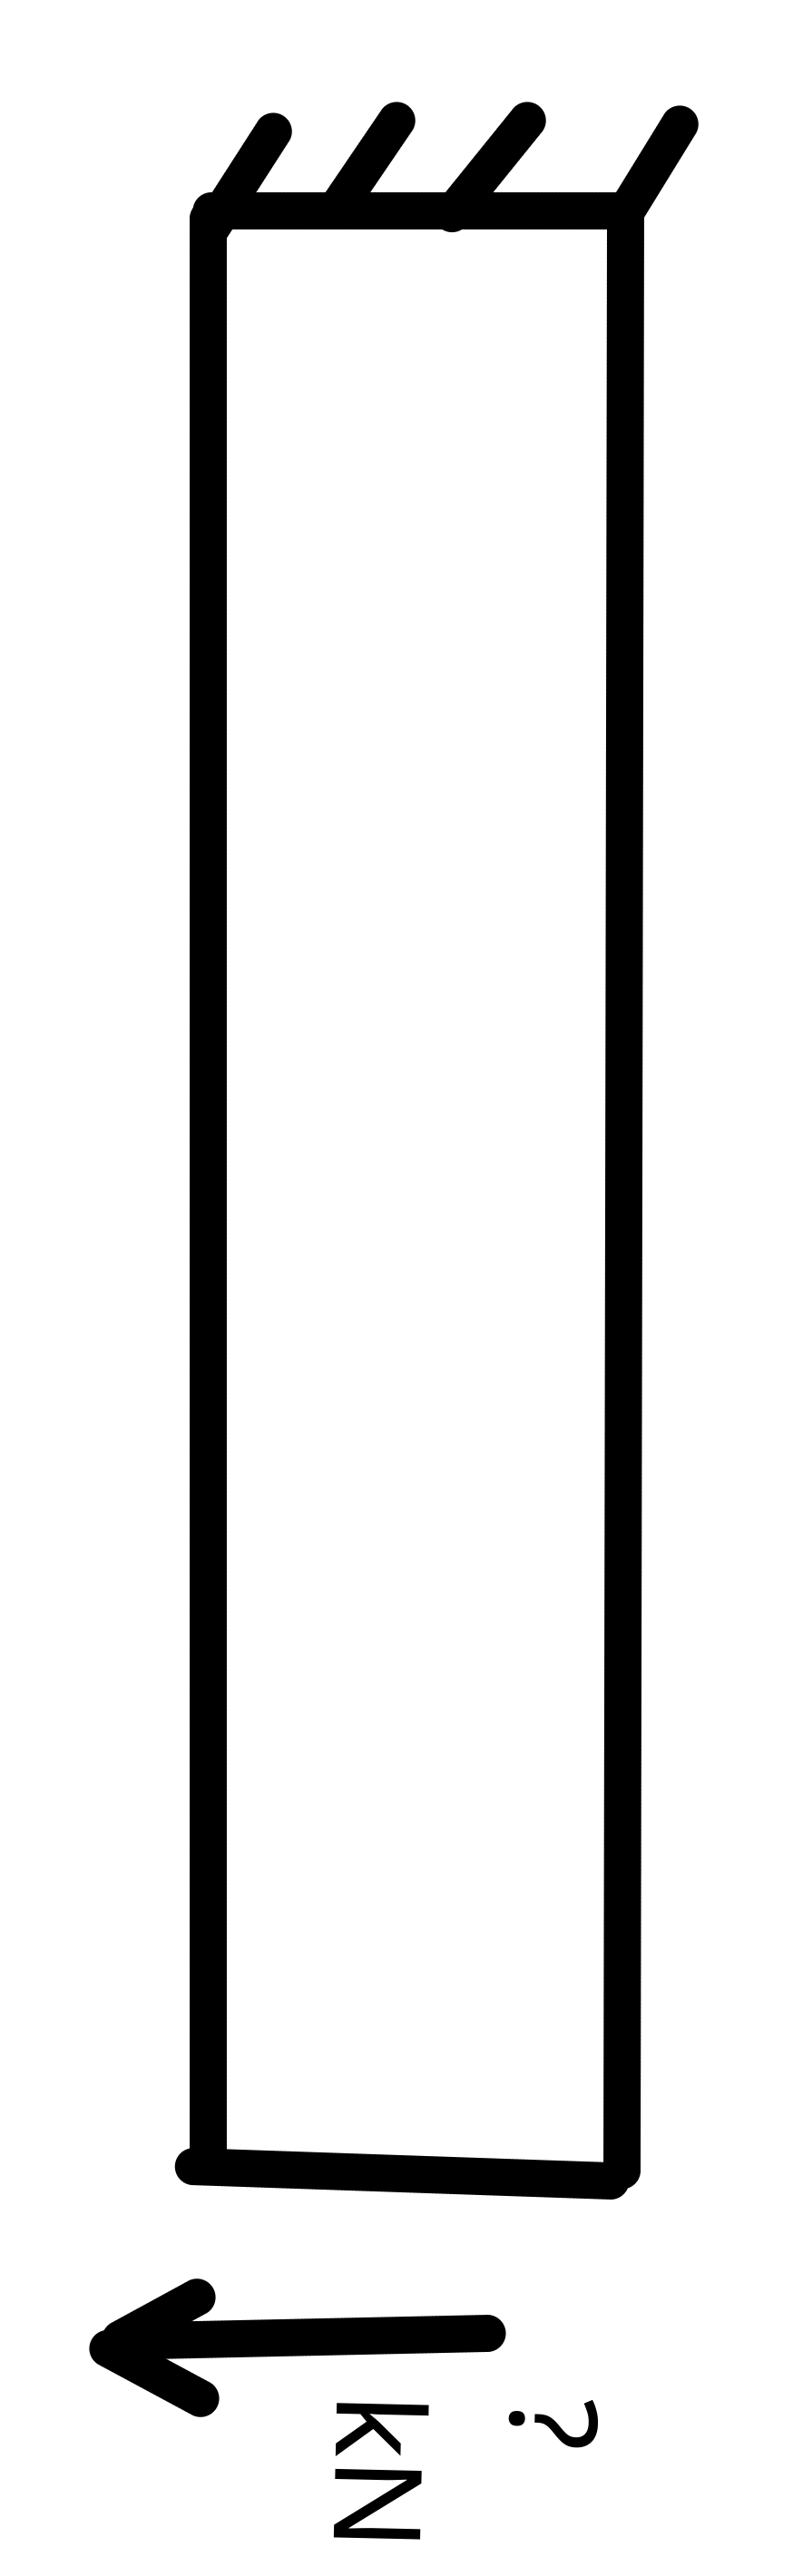
\includegraphics[width=0.3\linewidth,angle=90]{simplifiedcase}
		\caption{Caso simplificado. L = 4, ancho= 0.2, profundidad = 0.4 [m]}
		\label{fig:simplifiedcase}
	\end{figure}
\end{frame}

\begin{frame}{¿Qué nos hemos ahorrado?}
	\begin{itemize}[label=$\checkmark$]
		\item Condiciones de contacto en las planchas y los tornillos. No es necesario realizar un análisis \textbf{no lineal}
		\item Mucha geometría. No modelamos las planchas ni la soldadura
		\item Diferentes materiales tanto para los tornillos como para la soldadura
	\end{itemize}
	Además, nuestro caso tiene solución analítica, podemos comprobar los resultados
\end{frame}

\subsection{Geometría y grupos}

\begin{frame}{Comentarios sobre la geometría}
	\begin{itemize}
		\item Nombrad todo de forma comprensiva
		\item Es posible que queráis parametrizar algunos valores
		\item Sed lo más limpios posibles y concisos
	\end{itemize}
	\begin{block}{Grupos geométricos}
		Son elementos sobre los que nos apoyaremos para hacer el mallado y la simulación. Son zonas de \textbf{condiciones de contorno, cargas} y referencias.
	\end{block}
\end{frame}

\begin{frame}{Simplificaciones geométricas I}
	\textit{Una image vale más que mil palabras.} \\~
	
	Todas las imágenes de las secciones de geometría y mallado están tomadas del libro ``Finite element applications A practical guide to the FEM process''	
\end{frame}

\begin{frame}{Simplificaciones geométricas II}
	\begin{figure}
		\centering
		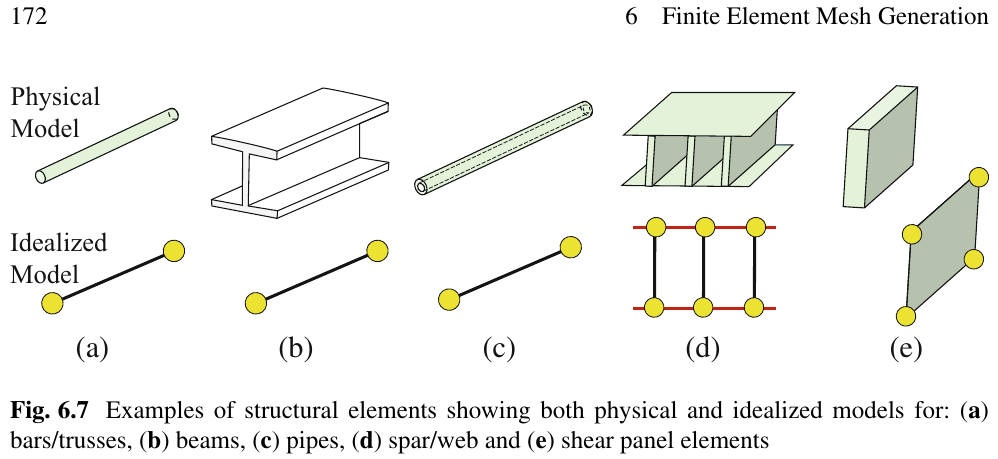
\includegraphics[width=1\linewidth]{real_idealised_mesh}
		\caption{Simprlificación real en modelos idealizados}
		\label{fig:realidealisedmesh}
	\end{figure}
\end{frame}

\subsection{Mallado (meshing)}

\begin{frame}{Información general}
	En resumidas cuentas, el mallado, \textit{meshing} en inglés, es la discretización espacial del problema en nodos, aristas y/o superficies/volúmenes. 
	Es de los temas más complicados y extensos que hay en la simulación FEM, después de todo, es lo que le da el nombre.
	
	\begin{block}{Nociones generales básicas}
		\begin{itemize}
			\item Tiene que permitir modelar el fenómeno físico, ver caso de la capa límite/viscosa
			\item Tiene que asegurar convergencia
			\item Tiene que asegurar precisión
			\item Tendría que ser sencillo
			\item Tendría que ser eficiente
		\end{itemize}
	\end{block}
\end{frame}

\begin{frame}{Ejemplos de referencia}
	\begin{figure}
		\centering
		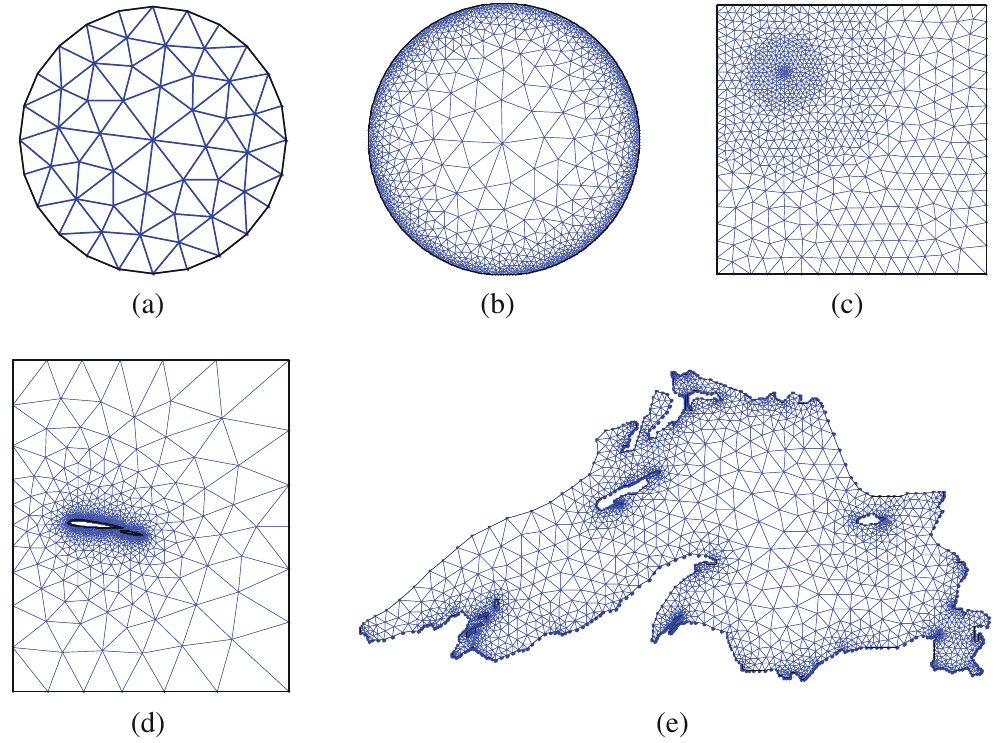
\includegraphics[width=0.9\linewidth]{mesh_refinement}
		\caption{Refinamiento por geometría}
		\label{fig:meshrefinement}
	\end{figure}
\end{frame}

\begin{frame}{Refinamiento del mallado}
	\begin{figure}
		\centering
		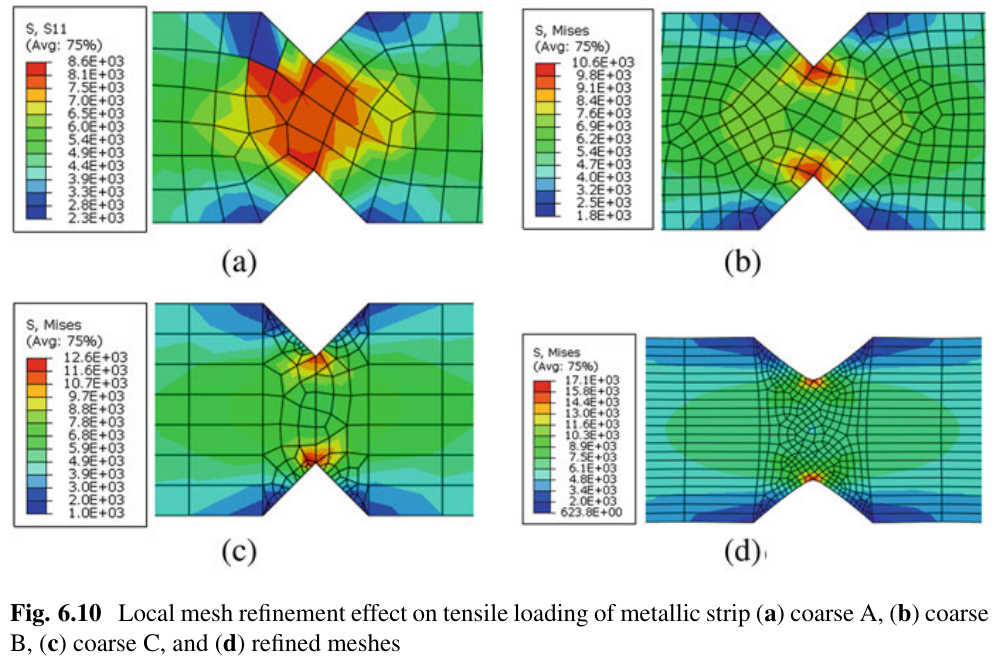
\includegraphics[width=0.9\linewidth]{mesh_refinement_steps}
		\caption{Evolución de la precisión por el refinamiento del mallado. Caso de concentración de tensiones}
		\label{fig:meshrefinementsteps}
	\end{figure}
	
\end{frame}

\begin{frame}{Unos sencillos pasos}
	Esta siguiente lista está hecha con SALOME en mente, pero otro software seguirá principios similares.
	\begin{enumerate}
		\item Importar geometría
		\item Discretizar de manera ``bruta'' (3D, 2D...)
		\item Seleccionar referencias
		\item Controlar la discretización con las referencias
		\item Recomputar
		\item (Re)hacer los grupos geométricos
		\item \textbf{Comprobar que todo esté correcto.} Por ejemplo: en CFD que los cuerpos sumergidos estén sellados
	\end{enumerate}
\end{frame}

\subsection{Simulación}

\begin{frame}{Nociones generales}
	En general, hay mil tipos de simulación: FE, por partículas, eventos discretos, formas analíticas, por frecuencias, integradores... \\
	Pero en FEM existe, de forma básica, estas categorías:
	\begin{itemize}
		\item Lineares y no lineares
		\item Transitorios o \textit{steady-state}
		\item Estáticos y dinámicos
		\item Modales, fatiga, fractura, térmica conjugada...
		\item Con o sin acoplamiento: termo-mecánico, termo-fluido...
	\end{itemize}
\end{frame}

\subsubsection{Fases generales de la simulación}

\begin{frame}{Secuencia para el diseño de una simulación}
	Esta lista está basada en el funcionamiento de SALOME-Meca, pero todo el software funciona igual:
	\begin{enumerate}
		\item Importar geometría
		\item Selección del tipo de simulación
		\item ``Diseñar'' materiales
		\item Asignar materiales a la geometría
		\item Asignar condiciones de contorno
		\item Asignar cargas
		\item Configurar la simulación
		\item Configurar la salida de datos y el post-procesado
	\end{enumerate}
	En cualquier momento puede ser necesario el uso de \textbf{funciones y listas de valores.} 
\end{frame}

\subsection{Post-procesado}

\begin{frame}{Nociones generales}
	El post-procesado es un sinónimo de \textbf{análisis.} ¿Qué se ha de hacer/suele hacer? 
	\begin{itemize}
		\item Analizar los resultados de la simulación
		\begin{itemize}
			\item ¿Son corréctos/esperados?
			\item El \textit{output} puede requerir de procesamiento extra, por ejemplo, \textit{plots}
		\end{itemize}
		\item Utilizar herramientas de filtrado
		\item Utilizar los resultados para derivar otros. Por ejemplo, con la presión que sufre un cuerpo desplazándose en un fluido, se puede procesas su coeficiente aerodinámico
	\end{itemize}
\end{frame}

\begin{frame}{Visualización geométrica de nuestra simulación}
	\begin{figure}
		\centering
		\hspace*{-1em}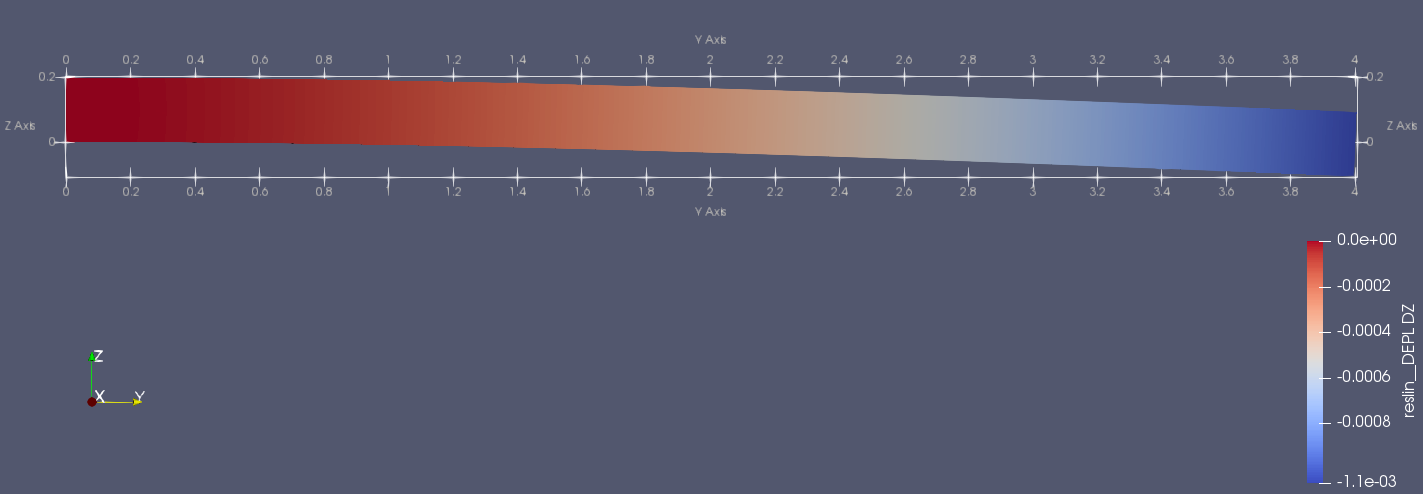
\includegraphics[width=1.1\linewidth]{3dview}
		\caption{Deformación vertical de la viga. Apliada 100 veces.}
		\label{fig:3dview}
	\end{figure}
\end{frame}

\begin{frame}{Visualización ``analítica'' de nuestra simulación}
	\begin{figure}
		\centering
		\hspace*{-1em}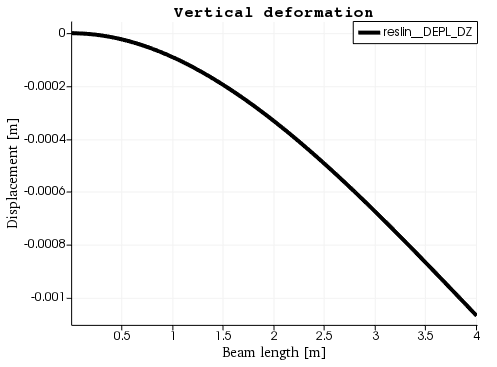
\includegraphics[width=1\linewidth]{postprodefline}
		\label{fig:lineresult}
	\end{figure}
\end{frame}

\begin{frame}{Fin}
	Recordad:
	\begin{itemize}
		\item Dad valor a la ingeniería
		\item Los cinco ``principios'' de la simulación
	\end{itemize}
	Recuerdo que tenéis listas de software para comparar y usar \\
	
	\textbf{Resultado analítico:} $\delta = 1.14\text{ [mm]}$
	
	\vfill
	\begin{center}
		\LARGE \textbf{¿Preguntas?}
	\end{center}
\end{frame}

\end{document}